\documentclass[12pt]{amsart}
\usepackage{amsmath,amssymb,url,color,tikz}
\usetikzlibrary{patterns} 
\usepackage[all]{xy}
\usepackage{young}
\usepackage{enumerate}
\usepackage[margin=1in]{geometry}
\usepackage{hyperref}
\usepackage{graphicx}
\usepackage{caption} 
\usepackage{subcaption}
\usetikzlibrary{arrows,automata}
\usepackage[colorinlistoftodos,color=red!70]{todonotes}

%\oddsidemargin = 0.0cm \evensidemargin = 0.0cm \textwidth = 6.5in
%\textheight =8.5in


\newtheorem{thm}{Theorem}
\newtheorem{lem}[thm]{Lemma}
\newtheorem{prop}[thm]{Proposition}
\newtheorem{cor}[thm]{Corollary}
\newtheorem{conj}[thm]{Conjecture}
\newtheorem{qn}[thm]{Question}

\theoremstyle{definition}
\newtheorem{defn}[thm]{Definition}
\newtheorem{ex}[thm]{Example}

\theoremstyle{remark}
\newtheorem{rem}[thm]{Remark}

\numberwithin{thm}{section}


\newcommand{\IMAGE}{\text{IMAGE}}
\newcommand{\LUT}{\text{LUT}}
%\newcommand{\RR}{\mathbb{R}}
%\newcommand{\ZZ}{\mathbb{Z}}
%\newcommand{\mcO}{\mathcal{O}}

\newcommand{\minho}[1]{\todo[color=yellow,inline]{minho: #1}}
\newcommand{\doyeob}[1]{\todo[color=blue!70,inline]{doyeob: #1}}
\newcommand{\mario}[1]{\todo[color=red,inline]{mario: #1}}
\newcommand{\emily}[1]{\todo[color=gray,inline]{emily: #1}}
\newcommand{\chensu}[1]{\todo[color=orange,inline]{chensu: #1}}
\newcommand{\morgan}[1]{\todo[color=green,inline]{morgan: #1}}
\newcommand{\chaiwah}[1]{\todo[color=pink,inline]{chaiwah: #1}}

\renewcommand{\qedsymbol}{$\blacksquare$}
\def\<{\langle}
\def\>{\rangle}
\def\longto{\longrightarrow}

\begin{document}


%\title{Team 4 (Fast and Somewhat Accurate Algorithms)}
\title{Fast and Somewhat Accurate Algorithms}

\author[Barela]{Mario Barela}
%, The University of Iowa}
\author[Chen]{Su Chen}
%, University of Kansas}
\author[Gunawan]{Emily Gunawan}
%, University of Minnesota}
\author[Schreffler]{Morgan Schreffler}
%, University of Kentucky}
\author[Song]{Minho Song}
%, Sungkyunkwan University
\author[Yeo]{Doyeob Yeo}
%, Korea Advanced Institute of Science and Technology (KAIST)}
\author[Wu]{Mentor: Chai Wah Wu (IBM), Team 4}

\address{Mathematical Modeling in Industry XIX (August 5-14, 2015)}

\date{\today}
\maketitle

%%=======================================
\section{Introduction}% and Problem Statement}
%%=======================================
In applications such as image processing, computer vision or image compression, often times accuracy and precision are less important than processing speed as the input data is noisy and the decision making process is robust against minor perturbations. For instance, the human visual system (HVS) makes pattern recognition decisions even though the data is blurry, noisy or incomplete and lossy image compression is based on the premise that we cannot distinguish minor differences in images. In this project we study the tradeoff between accuracy and system complexity as measured by processing speed and hardware complexity.

\section{Preliminary}
In image processing, an image is treated as a two-dimensional or three-dimensional matrix depending on whether the image is colored or grayscale. Through out this paper, an image will be denoted by its matrix representation $P$. For example, a colored image in the RGB mode whose size is $h\times w$ can be viewed as a three-dimensional matrix 
\[P=\{p_{ijk}\}_{h\times w\times 3}\] 
where  $i\in\{1,2,\dots,h\}$, $j\in\{1,2,\dots,w\}$ and $k\in\{1,2,3\}$, and for fixed $k$,
\[p_{ijk}\in\{0,1,,\dots,255\}\]
For simplicity, we only consider grayscale images in this paper so that the image is reduced to a two-dimensional matrix $P=\{p_{ij}\}_{h\times w}$ whose entries represents the pixel's intensity (0 for black and 255 for white). We will denote an $n\times n$ portion of the image $P$ by $P_n$. 

\subsection{Filtering images using convolution kernels}
A common task that is performed on an image is filtering them to achieve the desired result. For instance, a blurring filter, e.g. Gaussian blur filter, is introduced if we wish to smooth the skin of a person while an edge detection filter is applied for facial recognition problems. All of these filtering effects are obtained by convolving the image with a fixed matrix, which we call the \emph{convolution kernel} or \emph{filtering kernel} $K$. In most applications, $K$ is an $n\times n$ matrix ($n\ll h, n\ll w$) where $n$ is an odd number. In this paper, we will consider $3\times 3$ and $5 \times 5$ kernels.

The convolution of the image $P$ with kernel $K$, $P*K$, is a natural generalization of the familiar function convolutions. To be precise, let $P=\{p_{ij}\}_{h\times w}$ and $K=\{k_{ij}\}_{h\times w}$. Then $F=\{f_{mn}\}_{h\times w}\triangleq P*K$ is a matrix whose dimensional is the same as $P$ and the $mn$-th entry for $F$ is defined to be 
\[f_{m,n}=\sum_{i=-\infty}^{\infty}\sum_{j=-\infty}^{\infty}p_{i,j}\cdot k_{m-i,n-j}\]
where all non existent entries, e.g. $p[-1,-1]$, are treated as zero. Here we keep the dimension of $F$ as that of $P$ so that we can generate a filtered image with the same size. In practice, convolutions is done by first flipping the kernel $K$ and then sliding it along the image to get each output entry. 

\subsection{Measures of errors}\label{subsect:measures}
For the purpose of comparing two images, we need to introduce the following commonly used measures through which the accuracy of our algorithms are tested. All measures are based on a pixel by pixel evaluation. 
\begin{defn}
Let $A=[a_{ij}]_{h\times w}$ and $B=[b_{ij}]_{h\times w}$ be two image matrices. %we will define $\ell^2$-difference$(A,B)$ and $\ell^\infty$-difference$(A,B)$ by 
Define
\begin{align*}
\ell^2\text{-difference}(A,B) &:= \sqrt{ \frac{ \sum_{i,j} \left( a_{ij} - b_{ij} \right)^2} {h \times w}},\ \textrm{and}\\
\ell^\infty\text{-difference}(A,B) &:= \textrm{max}_{i,j} \left \vert a_{ij} - b_{ij} \right\vert.
\end{align*}
The peak signal-to-noise ration (PSNR) \cite{HG08} (in dB) is defined as
\begin{displaymath}
\begin{array}{ccl}
\textrm{PSNR}(A,B) & = & 10\cdot \textrm{log}_{10} \left( \frac{\textrm{MAX}_B^2}{\textrm{MSE}} \right)\\
		 & = & 20 \cdot \textrm{log}_{10} \left( \frac{\textrm{MAX}_B}{\sqrt{\textrm{MSE}}} \right)
\end{array}
\end{displaymath}
where
\begin{displaymath}
\textrm{MSE} = (\ell^2\text{-difference}(A,B))^2 \qquad \textrm{and} \qquad \textrm{MAX}_B= 255.
\end{displaymath}
Finally, the \emph{Image Euclidean Distance (IMED)} is given by
\[d_\text{IMED}^2(A,B) = \frac{1}{2\pi}\sum_{i,k = 1}^h\sum_{j,\ell = 1}^w \exp\left(\frac{-(k^2+\ell^2)}{2}\right)\big(a_{ij}-b_{ij}\big)\big(a_{i+k,j+\ell} - b_{i+k,j+\ell}\big).\]
\end{defn}

\begin{rem}
In general, $\text{MAX}_B$ is the maximum \emph{possible} pixel value of an image. Since we are assuming each pixel is an 8-bit integer, $\text{MAX}_B$ will be 255 for our purposes.
\end{rem}

\begin{rem}
PSNR can be easily calculated by using MATLAB command $\textrm{psnr}(A,B)$.
PSNR is the abbreviation for Peak Signal-to-Noise Ratio. In brief, it is a measurement of how much two images differ. A higher PSNR indicates smaller discrepancy between two images and two identical images has PSNR as $\infty$. Typical values for the PSNR in lossy images are between 30 and 50 dB, provided the bit depth is 8 bits. 
\end{rem}


\begin{rem}
See \cite{FWZ05} for an analysis of why IMED might be a reasonable image distance. Another reasonable image distance may be $\frac{d_\text{IMED}}{\sqrt{h\cdot w}}$.
\end{rem}

% \section{Challenges}
% On Wednesday August 5, we
% decided that look-up tables  are not suitable for a median filter algorithm.

% Although high-pass filters seem to respond well to truncation, blurring filter does not respond well to truncation.

\section{Look up tables and size reduction schemes}\label{section: look up table}

\subsection{Look-up tables (LUTs)}
The main computational cost of filtering an image lies in the process where we slide the convolution kernel and perform algebraic operations pixel by pixel. This will lead to huge amount of implementation time for pictures with large size nowadays. As in \cite{WSLQE06}, 
%discusses fast algorithms using look-up tables (LUT).
the usage of look up tables %(LUTs) 
provides a way to reduce the implementation time caused by direct algebraic computations. By storing the values of convolution of all possible square matrices with the fixed kermel matrix $K$, the look up table serves as a dictionary whose values can be retrieved readily:   
$$
\begin{bmatrix}
x_1 & x_2 & x_3\\
x_4 & x_5 & x_6\\
x_7 & x_8 & x_9
\end{bmatrix}
*
\begin{bmatrix}
k_1 & k_2 & k_3\\
k_4 & k_5 & k_6\\
k_7 & k_8 & k_9
\end{bmatrix}
\longrightarrow
\begin{bmatrix}
y_1 & y_2 & y_3\\
y_4 & y_5 & y_6\\
y_7 & y_8 & y_9
\end{bmatrix}
$$

The potential challenge for LUTs lies in their size which can be so large that storing them in the computer memory becomes impractical. As an example, a $3\times 3$ kernel $K$ with all entries non-zero will require $S=(2^8)^9=2^{72}$ bytes of memory, which is far beyond the storing capability of modern computers. In the subsections that follow, we will present several schemes where we use truncated look up tables with relatively small size. The performance of the truncated filter with LUTs and the resulting error will be studied in section \ref{section: numerical results}. 

\subsection{Bit Truncation}\label{subsection:bit_truncation}
One way to reduce the size of LUTs is to use truncated versions of the LUTs. Namely, we drop a prescribed number of bits from the entries in the square matrix that will be convolved with the kernel. Note that we do not truncate the convolution kernel. As an illustration of bit truncation, a binary number $11111011$ will become $11111000$ after we drop the last two digits, i.e. replacing them by $0$'s. In this case, the original set $\{0,1,\dots,255\}$ is turned into the set $\{0,4,8,12,\dots,252\}$ after the truncation by two bits. For notational convenience, we introduce the truncation matrix as follows:

\begin{defn}\label{defn:truncation_matrix}
Given an $n\times n$ filter kernel $K$, we say that an $n\times n$ matrix $T= \{t_{ij}\}_{n\times n}$ is a \emph{truncation matrix} or \emph{truncation scheme} if all its entries are integers from 0 to the image's bit depth. When performing a kernel convolution on an $n\times n$ block $P_n$ from an image with matrix $P$, $T$ indicates that we truncate the last $t_{ij}$ bits from the $ij$th entry of $P_n$ when applying $K$. 
\end{defn}

To make this clear, let
$$
T=
\begin{bmatrix}
1 & 2& 1\\
1 & 4 & 1\\
1 & 2 &1
\end{bmatrix}, \ \ \ 
P_n=
\begin{bmatrix}
p_1 & p_2& p_3\\
p_4 & p_5 & p_6\\
p_7 & p_8 &p_9
\end{bmatrix}
$$
This means that we will truncate that last $1$ bit from the $p_1$, $2$ bits from $p_2$, $3$ bits from $p_3$ and so on. It is easy to see that if $T_\text{tot} := \sum_{i,j=1}^nt_{ij}$, the size of the LUT associated with $K$ is reduced by a factor of $2^{T_\text{tot}}$ when truncated according to $T$.

Observe that truncations trade LUT size for algorithmic accuracy. Indeed, given some integer $0\le x\le 255$ with $x \equiv 0\ (\!\!\!\mod\ 2^{t_{ij}})$, if the $ij$th entry of $P$ is in the interval $[x,x+2^{t_{ij}}-1]$, it will still be entered into the LUT as $x$. If $t_{ij}$ is close to the bit depth of $\text{IMAGE}$, or if pixel values tend to be closer to the right endpoints of these intervals than to the left, this could potentially result in some fairly large error. 

Although the truncation scheme is able to reduce the size of LUTs substantially, it is still not enough to generate LUTs which are acceptable in practice, especially for LUTs constructed for low pass filters with 5 by 5 or even larger kernels. In what follows, we seek various decompositions of the kernel so that the LUTs for each decomposition matrix is small enough to be generated and stored in the memory. 

\subsection{A rank 1 decomposition}\label{rank 1 decomposition}

We first examine the simple case when $rank(K)=1$ where $K\in \mathbb{R}^{n\times n}$ and $n$ is an odd number. It is well known that every rank 1 matrix can be decomposed as
\[K=b\cdot c^T\]
for some $b,c\in \mathbb{R}^{n\times 1}$. The following relationship can be verified directly: 
\[K=b\cdot c^T=b*c^T\]
So is the equation
\begin{equation}\label{decomposition}
P*K=P*(b\cdot c^T)=P*(B*C)=(P*B)*C
\end{equation}
Here $B=(0,\dots,b,\dots,0)$ and $C=(0,\dots,c,\dots,0)$ where $0$ represents $n\times 1$ column vectors and $b$,$c$ are in the center ($n$ odd). We need to point out that (\ref{decomposition}) may not be true for general kernels which are not of rank one. This decomposition allows us to construct two LUTs for the kernel $K$, each of which is a table for the column vectors $b$ or $c$ since we can ignore all $0$'s. The size of LUTs are reduced significantly in this way.

As an example, let us consider the following low pass filter kernel
$$
K=\frac{1}{16}
\begin{bmatrix}
1 & 2 & 1\\
2 & 4 & 2\\
1 & 2 & 1
\end{bmatrix}
$$
It is apparent that $rank(K)=1$ and an obvious decomposition of $K$ is given by 
$$
K=\frac{1}{4}
\begin{bmatrix}
0 & 1 & 0\\
0 & 2 & 0\\
0 & 1 & 0
\end{bmatrix}*\frac{1}{4}
\begin{bmatrix}
0 & 0 & 0\\
1 & 2 & 1\\
0 & 0 & 0
\end{bmatrix}\triangleq B*C
$$
The symmetric decomposition of $K$ ($C=B^T$) simplifies the LUT further with only one LUT required, since
\[P*C=P^T*B\]
The normalizing constant $\frac{1}{4}$ rules out the possibility of overflow. The maximum size (no truncation) of the LUT is $(2^8)^3=2^{24}$ bytes, or 16MB. Truncation will further reduce the size to magnitude of kilobyte. Numerical test is given in subsection \ref{subsection:numerical_test_lowpass}. 
\subsection{Singular value decomposition}
Notice that the relationship (\ref{decomposition}) does not hold for general matrix $K$ even if $K$ can be decomposed as $K=B\cdot C$. However, any matrix can be written as the sum of a series of rank 1 matrices, i.e. we have the following singular value decomposition (SVD): 
\[K=\sum_{i=1}^{r}\sigma_i u_i\cdot v_i^T\]
Here $u_i$,$v_i\in\mathbb{R}^{n\times 1}$ are the left and right singular vectors respectively and $\sigma_i$ are singular values. Moreover, $u_i$'s and $v_i$'s compose of orthonormal matrices and $r$ is the rank of $K$. Now we are able to make use of the LUTs for rank 1 decomposition as in the previous section. As a result, at most $2r$ LUTs are required, each of which has a maximum size of $(2^8)^n=2^{8n}$ bytes. For example, a 3 by 3 kernel with rank 2 needs at most 4 LUTs with maximum size of 16Mb for each. The benefit of SVD is that for most kernels in practice, their rank (usually 1 or 2) is far less than their dimension so that very few LUTs are required even if the kernel has large dimensions. The other benefit we obtain from SVD lies in the fact that all the summands can be dealt with independently so that the power of parallel computation can be exploited. Singular value decomposition is the first generalization of the rank one decomposition in section \ref{rank 1 decomposition}. 
\subsection{Decomposition by rows}
The other generalization of rank one decomposition is achieved by splitting the rows. To be precise, let $K$ be an $n\times n$ filter kernel. For $k=1,\ldots,n$, let $e_k$ be the $n\times 1$ vector where $k$th entry is 1 and all other entries are 0, and let $r_k$ be the $k$th row of $K$. Note that $K$ may always be decomposed as 
$$K = \sum_{k=1}^nr_k * e_k$$
Taking advantage of the associativity of $*$ for vectors, it follows that 
$$K * P= \sum_{k=1}^nr_k * \left(e_k * P\right)$$
This is just another way of writing that summation is distributive, i.e.,
\[\sum_{q = (1-n)/2}^{(n-1)/2}\sum_{r = (1-n)/2}^{(n-1)/2}k_{i+q,j+r}p_{i-q,j-r} = \sum_{q = (1-n)/2}^{(n-1)/2}\left(\sum_{r = (1-n)/2}^{(n-1)/2}k_{i+q,j+r}p_{i-q,j-r}\right).\]

If we plan to use lookup tables to compute a matrix convolution, this observation greatly reduces the amount of memory required. Indeed, rather than having a single LUT which takes $n^2$ inputs and contains $2^{8n^2}$ entries, we have $n$ LUTs (one for each row of $K$), each of which takes $n$ inputs and contains only $2^{8n}$ entries. Again when $n=3$ this is a tremendous saving of memory (with 8-bit entries, one 4-zebibyte ($2^{72}$) LUT versus three 16MB ($2^{24}$) LUTs).

Further, the multiple-LUT approach can be easily implemented, and at a lower cost than direct computation. Before filtering any pixels, rotate $K$ by $180^o$ about its center. Then, take an $n\times n$ submatrix $P_n$ of $P$ centered about the pixel to which you wish to apply the kernel. Now simply enter the $i$th row of $P_n$ into the LUT associated with $r_i$ for $i = 1,2,\ldots,n$, and add the results. Thus, if we make the naive assumption that lookups and additions are computationally equivalent, only $2n-1$ operations ($n$ lookups and $n-1$ additions) are required per pixel. Compare this to $n^2+2n-2$ operations ($n^2$ multiplications and $2(n-1)$ additions) per pixel using direct computation.

Finally, when combined with bit truncation, each LUT can be made even smaller at the cost of an extra $n^2$ truncation operations per pixel. Unfortunately, if truncation is assumed equivalent to lookups and additions, this is not much more efficient than direct computation, since it saves only one operation per pixel. However, if truncation is cheaper than lookups and/or addition (which is suspected to be the case), combining bit truncation with this particular LUT scheme will drastically reduce computation time when compared with direct computation.

As an example, choose an arbitrary $3\times 3$ kernel $K$ and a truncation matrix $T = \left[\begin{smallmatrix}5 & 5 & 5\\5 & 2 & 5\\ 5 & 5 & 5\end{smallmatrix}\right]$, using the $i$th rows of $K$ and $T$ to produce the $i$th LUT. The associated LUTs will have 512, 4096, and 512 entries respectively. Even if each entry uses double precision, only 20kB of memory is required to store the LUTs, which is small enough to fit into cache memory. However, 14 operations (5 to use the LUTs as described previously, and 9 truncations) are required per pixel, versus 13 for direct computation. 

\subsection{A Decomposition Approximation}
Recall that a rank one decomposition of our kernel $K$ has the form 
$$
K=b*c^T
$$
where $c,b \in \mathbb{R}^n$. This ends up with in two LUTs of size $2^{24}$ bytes instead of the full LUT of size $2^{72}$ bytes. This drastically reduces the size of the LUT before any truncation but it requires us to have a rank 1 kernel $K$. Notice that the reduction of LUT size is the fact that the fewer non-zero entries we have the decomposition matrix, the smaller the LUT size is. For example, the $b$ and $c$ have three non-zero entries for each in the $3\times 3$ kernel case, whereas $K$ has nine non-zero entries. This observation leads to another possible decomposition which is described as follows (Take the $3\times 3$ kernel for demonstration). 

Consider the decomposition of $K$ into:
$$K\approx A*B$$
where $A$ and $B$ are of the form
$$\label{general decomposition}
A
=
\begin{bmatrix}
a & b & 0\\
c & d & 0\\
e & f & 0
\end{bmatrix}
,
B=
\begin{bmatrix}
g & h & i\\
j & k & l\\
0 & 0 & 0
\end{bmatrix}$$
\\
Note that there are only 6 non-zero entries for both $A$ and $B$. As a consequence, we are able the break the original $2^{72}$ bytes LUT into two LUTs of size $2^{48}$ bytes. In general this decomposition is not exact but we can find an approximated decomposition by posing this as a minimization problem. That is, we are looking for the solution of the following problem: 
$$\min \|K-A*B\|_F$$
Notice that there are other ways that we arrange the variables $a,b,..,l$ in the matrices $A$ and $B$. There are in fact $C_9^6$ possibilities for each of the two matrices. This gives us a total of  $(C_9^6)^2 =84^2= 7056$ possible minimization problems to solve. This seems like quite a lot of computation but this problem will actually be incorporated as a part of pre-processing. It is worth noting that some of the minimizing values in $(a,b,c,...,k,l)$ may be 0, which allow us to further reduce LUT size. For example, the decomposition may lead to $A$ having only 2 nonzero entries and $B$ with 4 nonzero entries. This would lead to two LUTs of size $2^{16}$ and $2^{32}$ bytes respectively.

We can actually change the structure of the matrices $A$ and $B$ above to have a variable amount of nonzero entries in them. This will allow us to force more entries in the matrices to be zero, resulting in smaller LUTs. 
\\
\textbf{Note:} After solving all possible minimization problems for a particular decomposition we will have a vector \textit{$f_{min}$} and a matrix \textit{$x_{min}$} containing all the min function values and minimizers. To get the ``best'' decomposition we look at the smallest function value. Since this will be an approximated decomposition, we should look at all function values under certain threshold and find the corresponding minimizers with the most zeros in it. For example, there may be two function min values smaller than $\min(f_{min}) + 10^{-2}$ with minimizers $x_1=(1, 3, 0, 4, 2, 1)$ and $x_2=(0, 0, 0, 1, 2, 0)$. In this case we should choose the minimizer $x_2$ because it has more zeros in it. It should also be noted that minimizers may have very small values which may be truncated. 

\textbf{Note:} We can reduce the number of non-zero entries in $A$ or $B$, but the corresponding decomposition errors may be too large for constructing a look up table. 

\textbf{Note:} If we build up look up tables with this kind of decomposition, we will introduce errors even if we do not truncate any bits, since the decomposition is not exact in most cases.

\subsection{Complement convolution kernels}
The last scheme we introduce in this paper is to take advantage of the complement convolution kernels. Tow convolution kernels $L$ and $H$ are called complement to each other if 
$$L+H=I$$
where $I$ is the identity matrix for convolution. Let $L(T)$, and $H(T)$ denote $L$ and $H$ with the truncation matrix $T$. Here we slightly abuse the notation since the truncations are made on the image, rather than the convolution kernels. After the bit truncation as in section \ref{subsection:bit_truncation}, we should have $H\approx H(T)$. As a result, we have 
$$L = I - H \approx I - H(T)$$.
Since $I = L + H$, we have $L = I - H \approx I - H(T)$. If we have constructed a look up table for the kernel $H$ with truncation scheme $T$, it can be used readily for the kernel $L$ since $P*I=P$. 

\section{Numerical results}\label{section: numerical results}
In this section, we implement the ideas in section \ref{section: look up table}. The filters we consider here includes $3\times 3$ blurring filter (a low pass filter), edge detection filter and Sobel magnitude edge-detection filter (high pass filters). The errors from the truncated look up tables are calculated with the measure introduced in subsection \ref{subsect:measures}. 
\subsection{A numerical test for blurring filter}\label{subsection:numerical_test_lowpass}
Consider the blurring filter kernel 
$$
K_1=\frac{1}{16}
\begin{bmatrix}
1 & 2 & 1\\
2 & 4 & 2\\
1 & 2 & 1
\end{bmatrix}
=
\frac{1}{4}
\begin{bmatrix}
0 & 1 & 0\\
0 & 2 & 0\\
0 & 1 & 0
\end{bmatrix}*\frac{1}{4}
\begin{bmatrix}
0 & 0 & 0\\
1 & 2 & 1\\
0 & 0 & 0
\end{bmatrix}\triangleq B*C
$$
As mentioned above, one look up table needs to be generated for kernel $K_1$. The truncation matrices we use are $T_1$ and $T_2$ where
$$
T_1=
\begin{bmatrix}
0 & 2 & 0\\
0 & 1 & 0\\
0 & 2 & 0
\end{bmatrix}
,\ \ \ \ \ \ T_2=
\begin{bmatrix}
0 & 4 & 0\\
0 & 2 & 0\\
0 & 4 & 0
\end{bmatrix}
$$
Here the numbers in matrices $T_1$ and $T_2$ are those of the bits to be truncated. Filtered images with direct computations and truncated LUTs are shown in figure \ref{fig:motor}. It is apparent that the blurred effect with truncated LUTs for the darker parts of the image is close to that obtained from direct application of the filter. There are visible artifacts for lighter parts of the image in the filtered images with truncated LUTs, which is an indication of a loss of precision after truncation. To measure the error introduced by our approximation, we will exploit the PSNR in subsection \ref{subsect:measures}. A comparison is summarized in Table \ref{tbl:low_pass}. The PSNRs for LUTs with $T_1$ and $T_2$ indicate that both schemes provides satisfactory approximation of the original filter. It is quite notable that even with truncation $T_2$, the PSNR is still above 30 with the size of LUT reduced to only 16Kb. 

We also run an optimization to examine which truncation scheme will give the best approximation of the original kernel, provided that the size of LUT is fixed at certain level. Some of the results are summarized in Table \ref{tbl:optimization}. It is not surprising that there is a symmetry in the best truncation scheme thanks to the symmetry of the original kernel $K_1$ . 

\begin{figure}[h] \centering 
\begin{subfigure}[b]{0.4\textwidth} 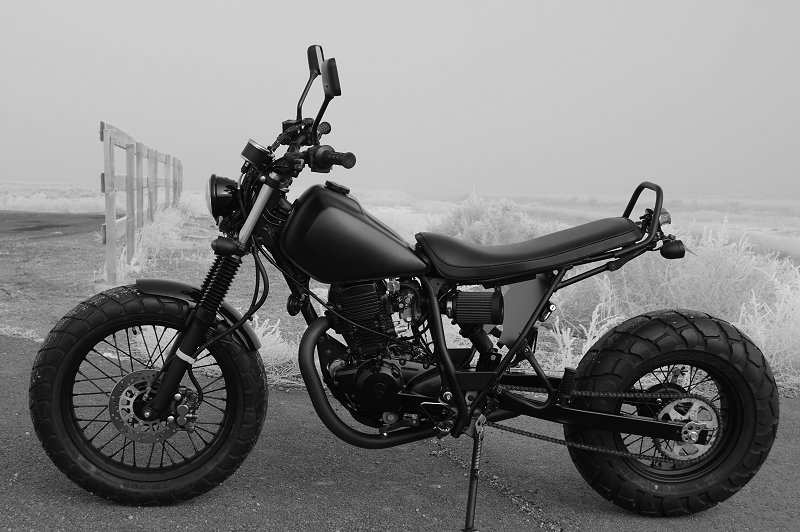
\includegraphics[width=\textwidth]{motor_original.png} \caption{Original image} %\label{fig:LPF} 
\end{subfigure}
\begin{subfigure}[b]{0.4\textwidth} 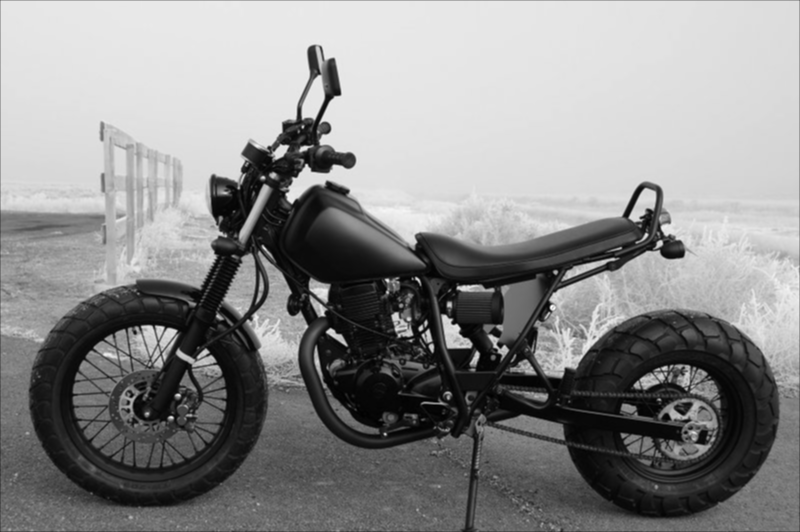
\includegraphics[width=\textwidth]{motor_direct.png} \caption{Low pass, direct}\end{subfigure}

\begin{subfigure}[b]{0.4\textwidth} 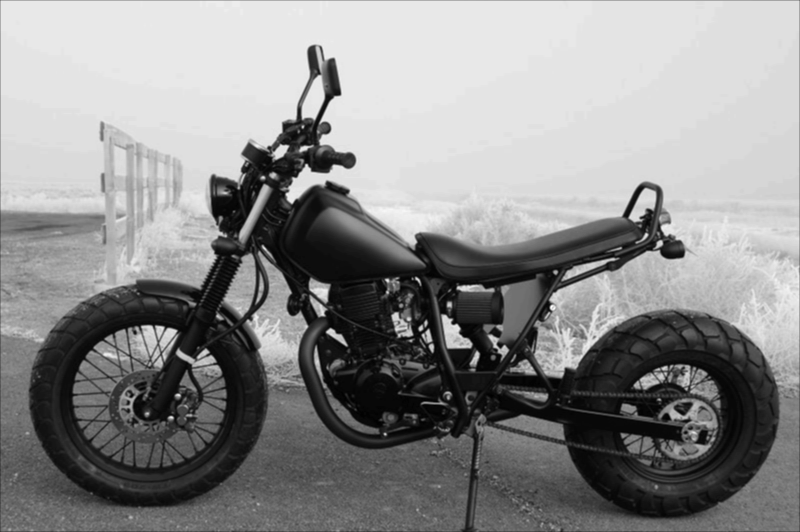
\includegraphics[width=\textwidth]{motor_lut_212.png} \caption{Low pass, LUT with $T_1$} %\label{fig:LPF} 
\end{subfigure}
\begin{subfigure}[b]{0.4\textwidth} 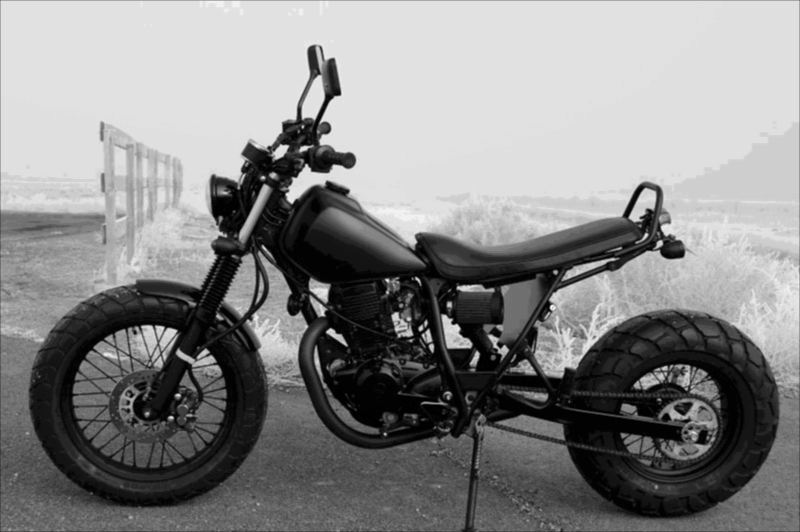
\includegraphics[width=\textwidth]{motor_lut_424.png} \caption{Low pass, LUT with $T_2$} \end{subfigure}
\caption{Comparison of filtered images. Figure A: The original image. Figure B: filtered image by direct applying kernel $K_1$. Figure C: filtered image by using LUT with truncation matrix $T_1$. Figure D: filtered image by using LUT with truncation matrix $T_2$}
\label{fig:motor} 
\end{figure}


\begin{center}
\begin{table}
	 
    \begin{tabular}{ | c | c| c |}
    \hline
    Scheme & LUT Size & PSNR (dB) \\ \hline
    Direct & N/A & N/A  \\ \hline
    LUT with $T_1$ & 512KB & 41.8459 \\ \hline
    LUT with $T_2$ & 16KB & 30.4442 \\ \hline   
    \end{tabular}
    \bigskip
    
    \caption{Error and size of LUT for direct computation and LUTs with different truncation schemes.}
    \label{tbl:low_pass}
\end{table} 
\end{center}

\subsection{A numerical test for edge detection filter}

The second numerical test involves the edge detection kernel (high pass filter)
$$
K_2=\frac{1}{8}
\begin{bmatrix}
-1 & -1 & -1\\
-1 &  8 & -1\\
-1 & -1 & -1
\end{bmatrix}
$$
\begin{center}
\begin{table}
	
    \begin{tabular}{ | c | c | c | }
    \hline
    LUT Size & Best Truncation & PSNR (dB) \\ \hline
    16Kb& $(0,b,0)$ with $b=(4,2,4)^T$ & 30.4442 \\ \hline
    32Kb& $(0,b,0)$ with $b=(3,3,3)^T$ & 33.3275 \\ \hline 
    64Kb& $(0,b,0)$ with $b=(3,2,3)^T$ & 35.5597 \\ \hline 
    256Kb& $(0,b,0)$ with $b=(2,2,2)^T$ & 39.4329 \\ \hline 
    \end{tabular}
    \bigskip
    
    \caption{Best truncation scheme for fixed-size LUT}
    \label{tbl:optimization}
\end{table} 
\end{center}

What this kernel does is to expose the edges of the pictures with white  color and the non-edges tend to be black. Evidently the rank of $K_2$ is 2 and we resort to the singular value decomposition approach for reduction of the look up table size. The decomposition is given by 
$$
K_2=U\Sigma V^T
$$
where
$$
U=
\begin{bmatrix}
 0.0971 & 0.7004 & -0.7071\\
-0.9905 & 0.1374 & 0\\
 0.0971 & 0.7004 & 0.7071
\end{bmatrix}
, \ \ \ \ \ \Sigma=
\begin{bmatrix}
1.0245 & 0 & 0\\
0& 0.2745 & 0\\
0 & 0 & 0
\end{bmatrix}
$$
and
$$
V=
\begin{bmatrix}
 0.0971 & -0.7004 & -0.7071\\
-0.9905 & -0.1374 & 0\\
 0.0971 & -0.7004 & 0.7071
\end{bmatrix}
$$

Four LUTs are needed since we need to deal with $u_1=(0.0971,-0.9905,0.0971)$, $u_2=(0.7004,0.1374,0.7004)$, $v_1=(0.0971,-0.9905,0.0971)$, $v_2=(-0.7004,-0.1374,-0.7004)$ separately. The increase in the number of LUTs causes the size of LUTs to rise. Another factor that contributes to the increase in the LUT size is the singular vectors which may stretch the original values of each pixel. As in the low pass filter, we still use the two truncation schemes $T_1$ and $T_2$ and the image we use here has the size $1024\times 768$. The filtered images with direct computation and truncated LUTs are shown in figure \ref{fig:house} while the errors in PSNR and the size of the LUTs are listed in Table \ref{tbl:high_pass}. 
Note that the size of LUTs are significantly larger than that of the rank one kernel $K_1$. We observe that the size with SVD is approximately 8 times, rather than 4, of the previous LUT for rank 1 case. The extra increase in the size is due to the stretching effect of singular vectors. However, by truncating more numbers of bits, such as the $T_2$ scheme, we can draw similar conclusions, as in the case of low pass filter, that our truncated LUTs with the SVD scheme provides satisfactory result while the size of the LUTs are kept small enough in practice. 

\begin{figure}[h] \centering 
\begin{subfigure}[b]{0.4\textwidth} 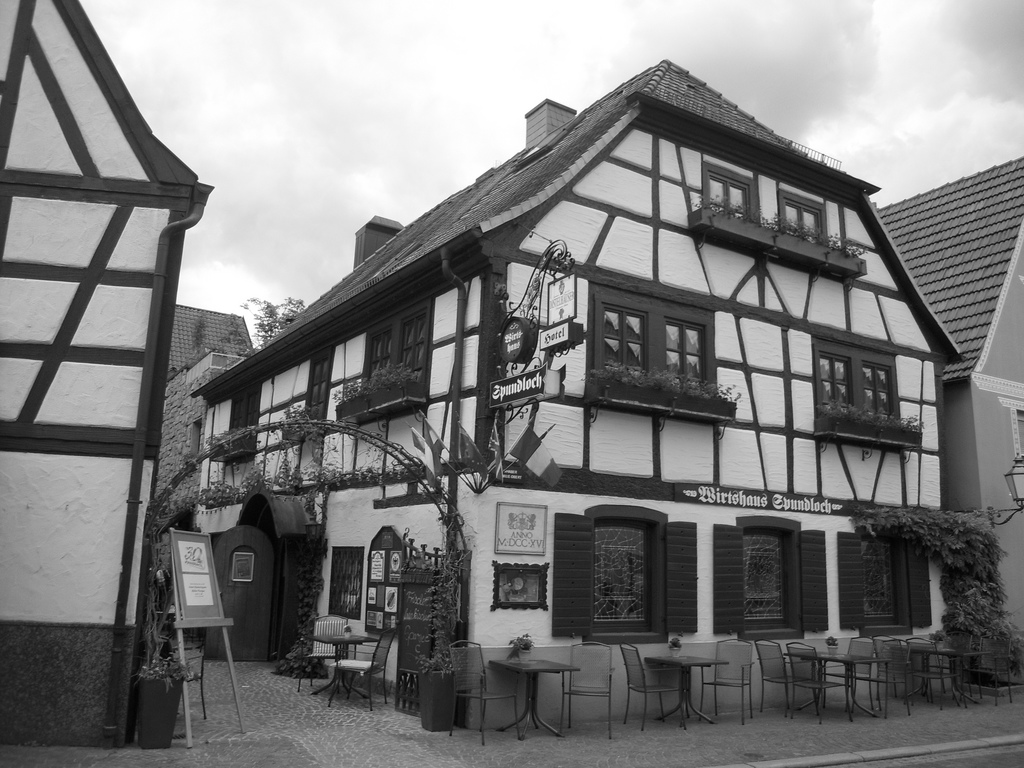
\includegraphics[width=\textwidth]{house_original.png} \caption{Original image} %\label{fig:LPF} 
\end{subfigure}
\begin{subfigure}[b]{0.4\textwidth} 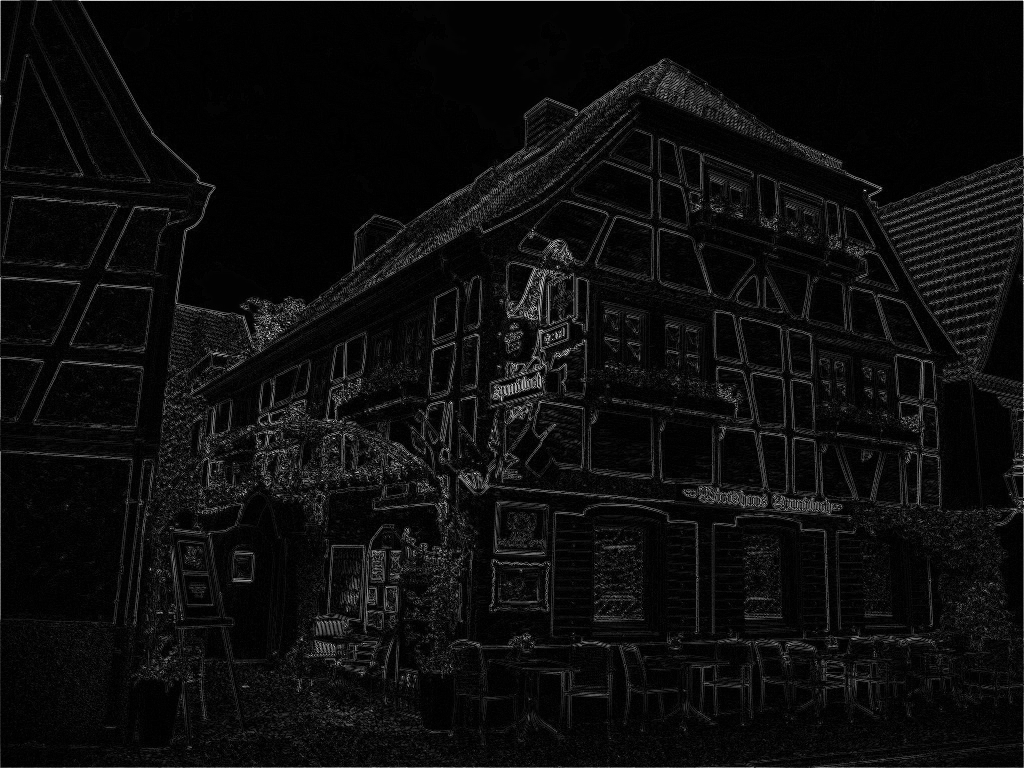
\includegraphics[width=\textwidth]{house_direct.png} \caption{Low pass, direct}\end{subfigure}

\begin{subfigure}[b]{0.4\textwidth} 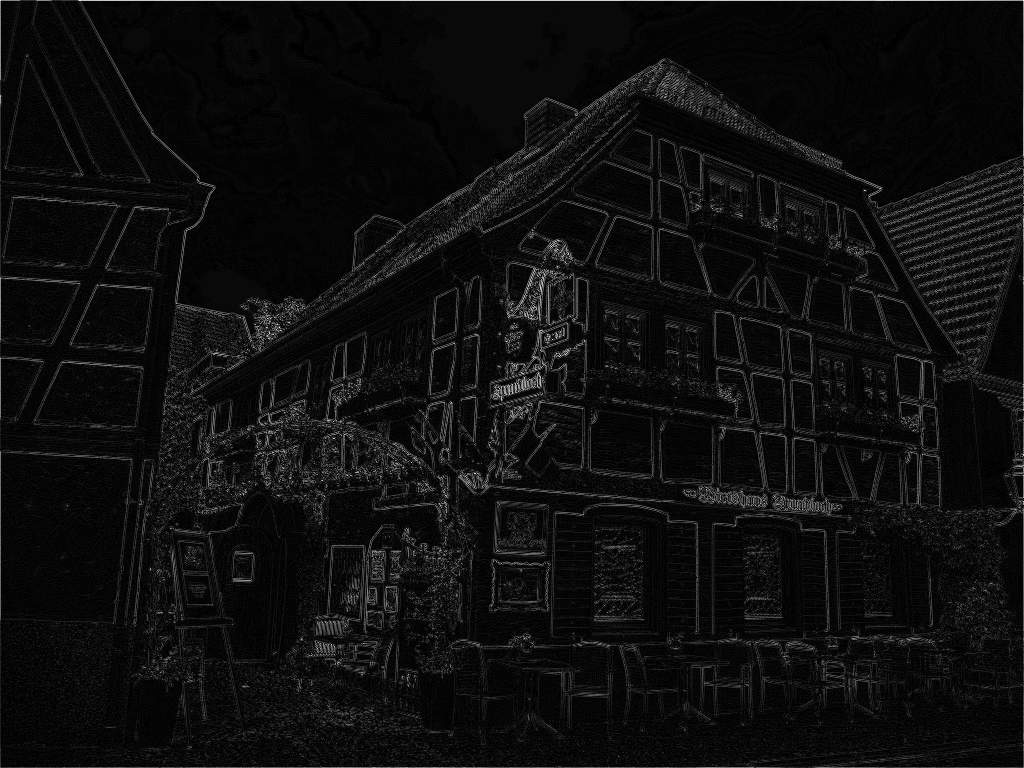
\includegraphics[width=\textwidth]{house_lut_212.png} \caption{Low pass, LUT with $T_1$} %\label{fig:LPF} 
\end{subfigure}
\begin{subfigure}[b]{0.4\textwidth} 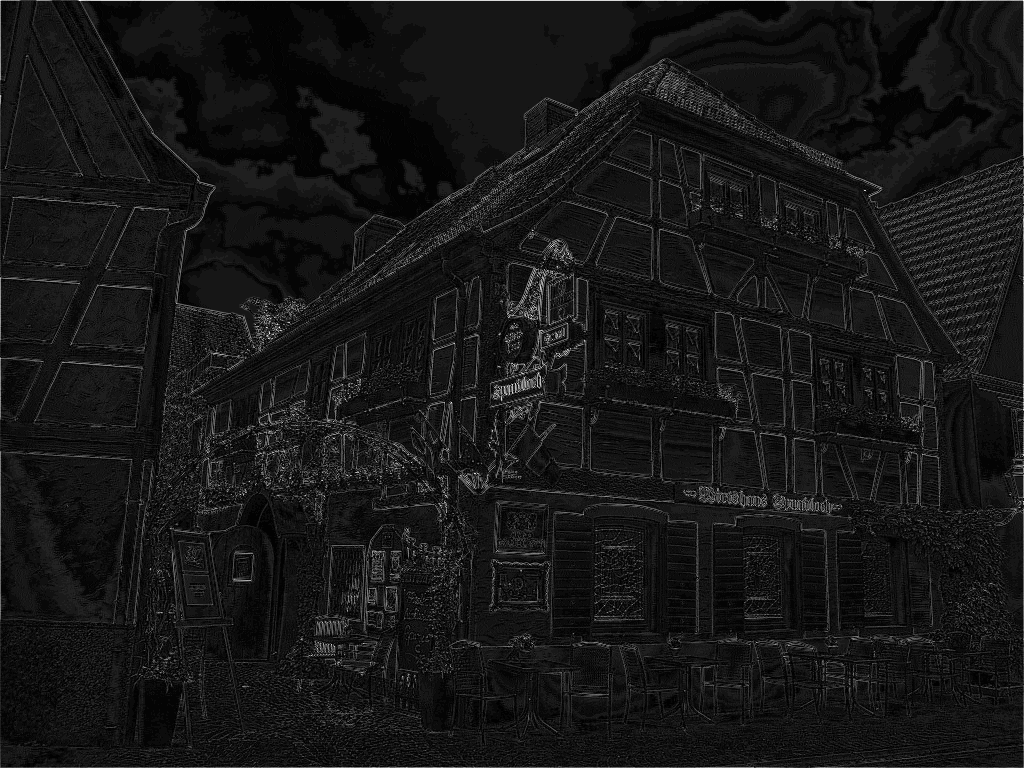
\includegraphics[width=\textwidth]{house_lut_424.png} \caption{Low pass, LUT with $T_2$} \end{subfigure}
\caption{Comparison of filtered images. Figure A: The original image. Figure B: filtered image by direct applying kernel $K_2$. Figure C: filtered image by using LUT with truncation matrix $T_1$. Figure D: filtered image by using LUT with truncation matrix $T_2$}
\label{fig:house} 
\end{figure}



\begin{center}
\begin{table}
	 
    \begin{tabular}{ | c | c| c |}
    \hline
    Scheme & Total LUT Size & PSNR (dB) \\ \hline
    Direct & N/A & N/A  \\ \hline
    LUT with $T_1$ & 3.8MB & 40.9868 \\ \hline
    LUT with $T_2$ & 128.8KB & 30.4436 \\ \hline   
    \end{tabular}
    \bigskip
    
    \caption{Error and size of LUT for direct computation and LUTs with different truncation schemes.}
     \label{tbl:high_pass}
\end{table}
\end{center}

\subsection{A numerical test for the Sobel magnitude edge-detection filter}\label{subsubsection:sobel}
We describe a numerical test using a similar method as in section \ref{rank 1 decomposition}. 
The Sobel gradient magnitude is an edge-detection operation \cite{Sob68} which can be computed using
$\mathbf{G} = \sqrt{ {\mathbf{G}_x}^2 + {\mathbf{G}_y}^2 }$
where
$$\mathbf{G}_x = P*\begin{bmatrix} 
 -1 & 0 & +1  \\
-2 & 0 & +2 \\
-1 & 0 & +1 
\end{bmatrix} 
\quad
\mbox{and}
\quad   
\mathbf{G}_y = P*\begin{bmatrix} 
-1 & -2 & -1 \\
 0 & 0 & 0 \\
+1 & +2 & +1
\end{bmatrix}$$
Let $$K_x=\begin{bmatrix} 
 -1 & 0 & +1  \\
-2 & 0 & +2 \\
-1 & 0 & +1 
\end{bmatrix}=
\begin{bmatrix}0 &1 &0\\0 &2 &0 \\0 &1 &0
\end{bmatrix}
\begin{bmatrix}0 &0 &0\\-1 & 0 & 1\\ 0 & 0 &0\end{bmatrix}$$ and
$$K_y=\begin{bmatrix} 
 -1 & -2 & -1  \\
0 & 0 & 0 \\
+1 & +2 & +1 
\end{bmatrix}=
\begin{bmatrix}0 &-1 &0\\0 &0 &0\\0 &1 &0
\end{bmatrix}
\begin{bmatrix}0 & 0 & 0\\ 1 & 2 & 1 \\ 0 &0 &0\end{bmatrix}.$$


%A full look-up table $\LUT(K_x)$ for $K_x$ requires $256^6$ bytes to store. In contrast, a look-up table $\LUT(K_x)(T)$ with truncation matrix $T= \begin{bmatrix} 
%5 & 8 & 5 \\
% 5 & 8 & 5 \\
%5 & 8 & 5
%\end{bmatrix}$ takes up $8^6$ bytes.



Let $T_j$ denote the truncation matrices
$\begin{bmatrix}
0 & j & 0\\
0 & j & 0\\
0 & j & 0
\end{bmatrix}
$ and 
$\begin{bmatrix}
0 & 0 & 0\\
j & j & j\\
0 & 0 & 0
\end{bmatrix}
$
where the numbers in matrices $T_k$ are those of the bits to be truncated. Because of the symmetry in the entries of $K_x$ and $K_y$, we can use the same look-up table, say, $\LUT(K_x)_T$, for both kernels. Let $\mathbf{G}(T)$ denote the Sobel magnitude operation using the truncated look-up table $\LUT(K_x)_T$.

To measure the error introduced by our approximations, we use the PSNR together with the two norms $\ell_2$ and $\ell_{\infty}$ introduced in subsection \ref{subsect:measures}. The comparison summarized in Table \ref{tbl:sobel} is done for a suite of representative images. The PSNRs and norms show that truncation up to $5$ digits provide satisfactory approximations to the actual Sobel magnitude operation.

The sizes of the LUTs for different truncation matrices $T_j$ are also listed in Table \ref{tbl:sobel}. The filtered images with direct computation and truncated LUTs are shown in figure \ref{fig:german_sobel}.
\begin{center}
\begin{table}
    \begin{tabular}{ | c | c | c | c | c | }
    \hline
    \hline
truncation &	LUT sizes	&PSNR 	&$\ell_2$ 	&$\ell_{\infty}$ \\ \hline
$T_0$&	16MB and 64KB		&$\inf$		&0	&0\\ \hline
$T_1$&	2MB and 16KB		&52.1,54.9	&$4.3 10^{-7}, 1.4 10^{-6}$	&0.00551,0.0086\\ \hline
$T_2$&	256KB and 4KB		&44.7,47.2	&$1.2 10^{-6}, 2.7 10^{-6}$	&0.0144, 0.0210\\ \hline
$T_3$&	32KB and 1KB		&38.3,40	&$2.6 10^{-6}, 5.4 10^{-6}$	&0.0310, 0.0423\\ \hline
$T_4$&	4KB	and 256 bytes	&32.4, 33.5	&$6.1 10^{-6}, 1.1 10^{-5}$	&0.0698, 0.0876\\ \hline
$T_5$&	512 bytes and 64 bytes &26.1, 27.7	&$1.3 10^{-5}, 2.8 10^{-5}$		&0.1443, 0.1714\\ \hline
 \end{tabular}
\caption{Ranges of PSNR and norms for a suite of images for measuring the difference between $\mathbf{G}(T_j)$ and $\mathbf{G}$. See Section \ref{subsubsection:sobel}}\label{tbl:sobel}
\end{table} 
\end{center}

\begin{figure}[h] \centering 
\begin{subfigure}[b]{0.4\textwidth} 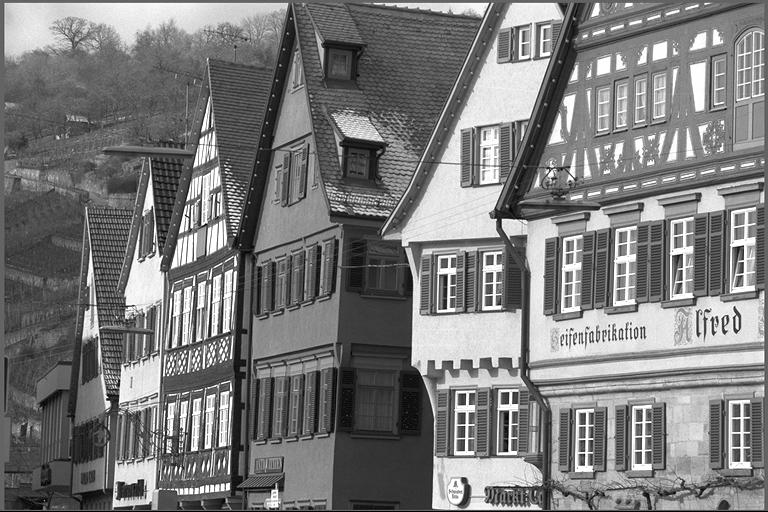
\includegraphics[width=\textwidth]{german.jpg} \caption{Original image} %\label{fig:LPF} 
\end{subfigure}
\begin{subfigure}[b]{0.4\textwidth} 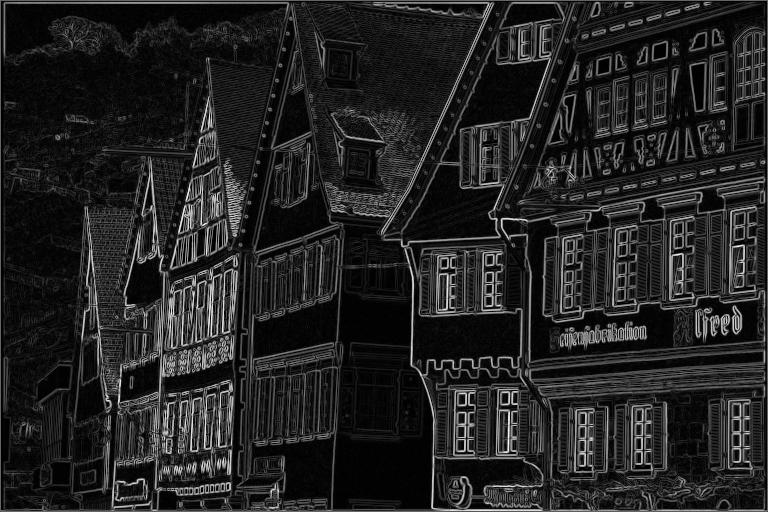
\includegraphics[width=\textwidth]{german0.jpg} \caption{Sobel magnitude, direct}\end{subfigure}
\begin{subfigure}[b]{0.4\textwidth} 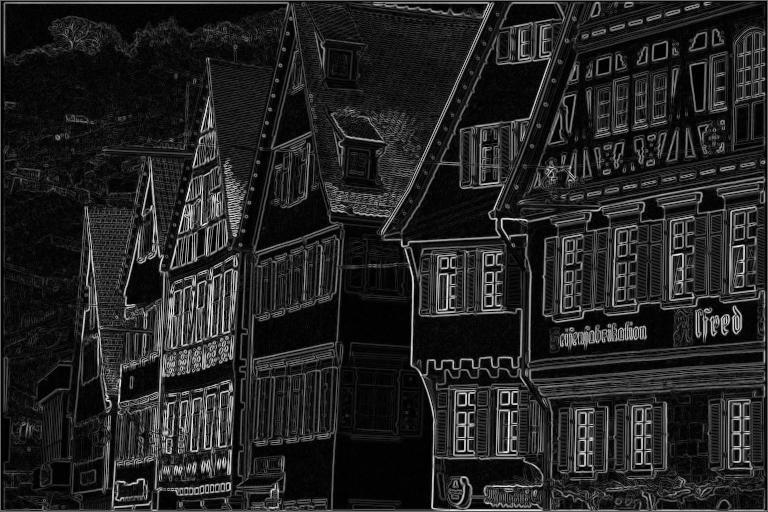
\includegraphics[width=\textwidth]{german1.jpg} \caption{Sobel magnitude, LUT with $T_1$} %\label{fig:LPF} 
\end{subfigure}
\begin{subfigure}[b]{0.4\textwidth} 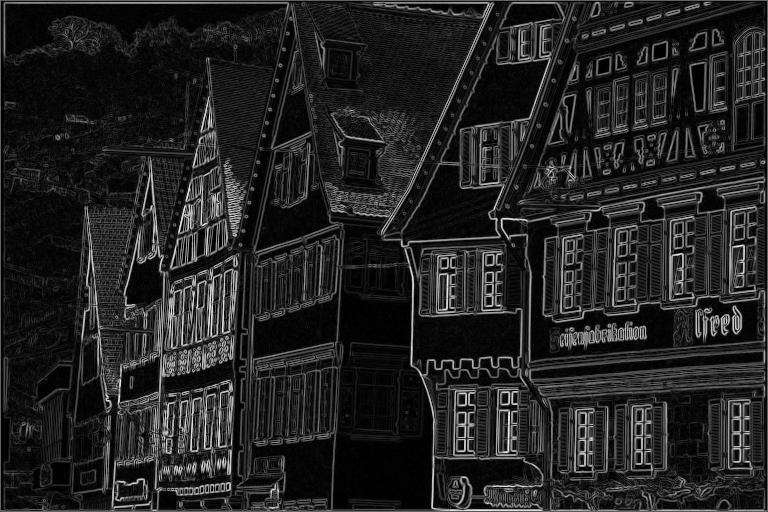
\includegraphics[width=\textwidth]{german2.jpg} \caption{Sobel magnitude, LUT with $T_2$} \end{subfigure}
\begin{subfigure}[b]{0.4\textwidth} 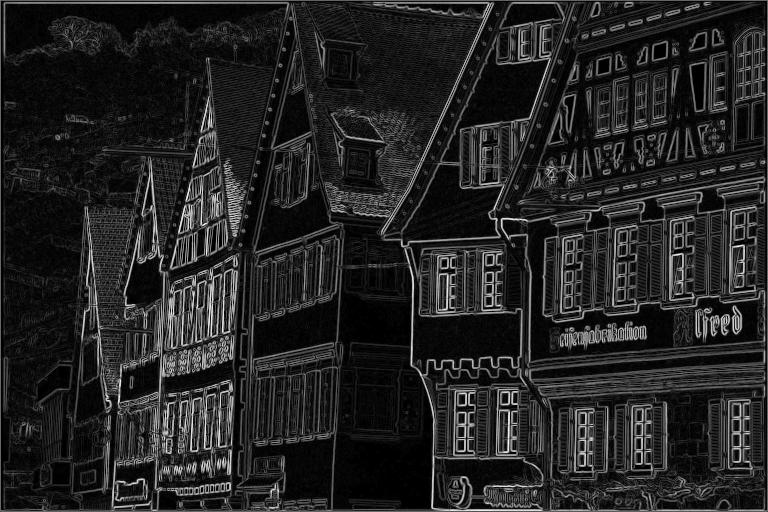
\includegraphics[width=\textwidth]{german3.jpg} \caption{Sobel magnitude, LUT with $T_3$} %\label{fig:LPF} 
\end{subfigure}
\begin{subfigure}[b]{0.4\textwidth} 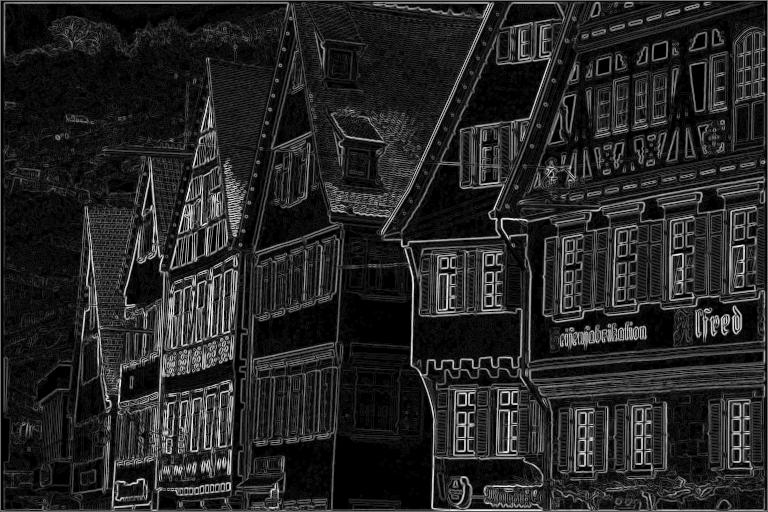
\includegraphics[width=\textwidth]{german4.jpg} \caption{Sobel magnitude, LUT with $T_4$} \end{subfigure}

\caption{Comparison of results of the Sobel magnitude operation with various truncation matrices. See Section \ref{subsubsection:sobel}.}
\label{fig:german_sobel} 
\end{figure}
\subsection{A numerical test for complement kernels}
In the following example, we will test the performance for the truncated look up tables with the complement kernel. Consider a high-pass filter
$$H=
\frac{1}{8}
\begin{bmatrix}
0 & -1 & 0\\
-1 & 4 & -1\\
0 & -1 & 0
\end{bmatrix}$$
and its complement (a low pass filter)
$$L=
\frac{1}{8}
\begin{bmatrix}
0 & 1 & 0\\
1 & 4 & 1\\
0 & 1 & 0
\end{bmatrix}$$
Let $$
T_{1}=\left[
\begin{array}{ccc}
8 & 4 & 8 \\
4 & 2 & 4 \\
8 & 4 & 8
\end{array}
\right] ,T_{2}=\left[
\begin{array}{ccc}
8 & 5 & 8 \\
5 & 3 & 5 \\
8 & 5 & 8
\end{array}
\right] \mbox{ and }T_{3}=\left[
\begin{array}{ccc}
8 & 6 & 8 \\
6 & 4 & 6 \\
8 & 6 & 8
\end{array}
\right]
$$
be three truncation matrices. We perform two truncated look up table schemes: the first one involves the LUT with $L(T_i)$ and the second one involves $I-H(T_i)$. The table \ref{table:comparison_of_errors} shows us how $L(T_i)$ and $I-H(T_i)$ are different from the low-pass filter $L=I-H$ for each $i$. In this table, $L(T_i)$ is denoted by Old and $I-H(T_i)$ is called New. 

\begin{table}[ht]
\begin{center}
\begin{tabular}{c|c|c|c|c|c|c|}
\cline{2-7}  & \multicolumn{2}{|c|}{$T_{1}$} &
\multicolumn{2}{c|}{$T_{2}$} & \multicolumn{2}{c|}{$T_{3}$}
\\\cline{2-7} & Old & New & Old & New & Old & New \\\hline \multicolumn{1}{ |c| }{PSNR} &
38.12 & 39.58 & 30.80 & 32.84 & 22.59 & 25.59 \\\hline
\multicolumn{1}{ |c| }{$l_{2}$ - error} & 3.06 &  2.80 &  7.40 & 5.87 &
18.87 & 13.52 \\\hline \multicolumn{1}{ |c| }{$l_{\infty
}$ -
error} & 8.42 & 7.40 & 19.64 & 15.81 & 43.35 & 35.70 \\
\hline
\end{tabular}
\bigskip

\caption{Comparison of errors}
\label{table:comparison_of_errors}
\end{center}
\end{table}
As you see, our new approach gives us the better results no matter which truncation matrix you use.
See also Figures \ref{fig:comp} made via the truncation matrix $T_3$.
\begin{figure}[h] \centering 
\begin{subfigure}[b]{0.3\textwidth} 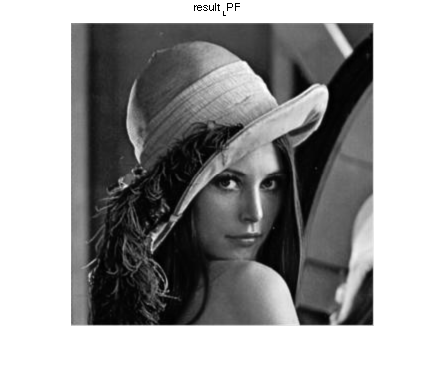
\includegraphics[width=\textwidth]{LPF.png} \caption{LPF} \label{fig:LPF} \end{subfigure}
\begin{subfigure}[b]{0.3\textwidth} 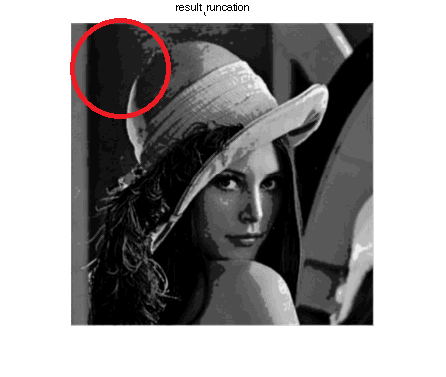
\includegraphics[width=\textwidth]{truncation.png} \caption{LPF with Truncation} \label{fig:LPF with Truncation} \end{subfigure}
\begin{subfigure}[b]{0.3\textwidth} 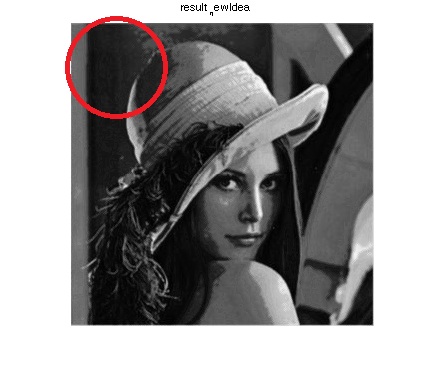
\includegraphics[width=\textwidth]{new.png} \caption{Result of the New Idea} \label{fig:new} \end{subfigure}
\caption{Comparison of filtered images}\label{fig:comp} 
\end{figure}

If we use the scheme $L\approx I-H(T_i)$, we can make use of the LUT for $H(T_i)$ directly. Surprising enough, the $I-H(T_i)$ scheme works even better than using the LUT with $L(T_i)$, indicating that the truncated look up tables are working better for high pass filters than the low pass filters. See also Figures \ref{fig:comp} made via the truncation matrix $T_3$ where the staircase effects are reduced with the application of complement scheme. 

\section{Conclution}
In this paper, we demonstrated the application of look up tables in image filtering where a pre-processed table are used to save the algebraic operations. The main challenge is to reduce the size of the look up tables for a given convolution kernel $K$. Several techniques are introduced to solve the size problem, including truncation, rank one decomposition, SVD, row decomposition, general decomposition and complement kernels. We perform several numerical tests to study the trade off between truncation and precision using those schemes and conclude that with the proper use of those schemes, a mild truncation scheme can result in both small errors for approximation of the direct calculation and a look up table that is small enough to stored in the computer memory. 



%Note that the second and third step stands for avoiding staircase effects.




\begin{thebibliography}{widest entry}
\bibitem[WSLQE06]{WSLQE06}
Wu, C. W., Stanich, M., Li, H., Qiao, Y., Ernst, L., "Fast Error Diffusion and Digital Halftoning Algorithms Using Look-up Tables," Proceedings of NIP22: International Conference on Digital Printing Technologies, Denver, Colorado, pp. 240-243, September 2006.


\bibitem[SF68]{Sob68}
Sobel, Irwin and Feldman, Gary,
{A 3x3 isotropic gradient operator for image processing}, 1968.
%{https://en.wikipedia.org/wiki/Sobel_operator}

\bibitem[HG08]{HG08}
Huynh-Thu, Quan and Ghanbari, Mohammed,
Scope of validity of PSNR in image/video quality assessment,
Electronics letters, vol. 44, no. 13, pp. 800-801, 2008.

\bibitem[FWZ05]{FWZ05}
Jufu Feng, Liwei Wang, Yan Zhang, "On the Euclidean Distance of Images," IEEE Transactions on Pattern Analysis and Machine Intelligence, vol. 27, no. 8, pp. 1334-1339, 2005.
\end{thebibliography}
 \end{document}